\documentclass[12pt, a4paper]{report}

\usepackage{amsmath}
\usepackage{amssymb}
\usepackage{amsthm}
\usepackage{hyperref}
\usepackage[parfill]{parskip}
\usepackage[linewidth=1pt]{mdframed}
\usepackage{graphicx}

\graphicspath{ {./images/} }

\hypersetup{
  colorlinks=false,
  linkcolor=black,
  filecolor=black,      
  urlcolor=black,
  pdftitle={Raccolta dimostrazioni CLF},
  pdfpagemode=FullScreen,
}

\mdfsetup{ skipabove=12pt, skipbelow=6pt }
\renewcommand{\contentsname}{Contenuti}


\title{Raccolta di appunti di Data e Web Mining}
\author{???}
\date{\today}

\begin{document}
  \maketitle
  \tableofcontents

  \chapter{Introduction}
\textbf{Cosa vuol dire fare Data Mining?}

Il data mining è il processo di scoperta automatica di informazioni utili in grandi basi di dati. Le tecniche di data mining vengono implementate per setacciare grandi insiemi di dati al fine di trovare modelli nuovi e utili per prevedere l'esito di un'osservazione futura.

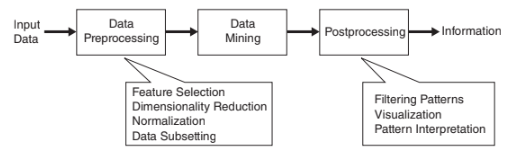
\includegraphics[width=10cm]{introduction.png}

I dati dati in input ad un algoritmo di data mining possono essere memorizzati in una varietà di formati (file flat, fogli di calcolo,
o tabelle relazionali) e possono risiedere in un repository di dati centralizzato o essere
distribuiti su più siti. 

\textbf{ Le fasi di un algoritmo di Data Mining sono:}

1)\underline{Data Preprocessing}

Durante questa fase i dati in input grezzi vengono trasformati, quindi vengono puliti dal rumore, vengono rimossi i duplicati
e vengono selezionate le variabili/feature più significative. Questo processo è quello più laborioso e dal quale dipende
poi tutta la successiva fase di estrapolazione dei modelli, se viene fatto male quindi l'intero processo è compromesso.

2) \underline{Data Postprocessing}

Durante questa fase solo i risultati validi e utili vengono tenuti per fare previsioni.
Un esempio di post-elaborazione è la visualizzazione, che consente agli analisti di esplorare i dati e i risultati da diversi punti di vista.
I metodi di verifica delle ipotesi possono essere applicati anche durante la post-elaborazione.

\textbf{Quali sono i task del Data Mining?}

Le attività di data mining sono generalmente suddivise in due categorie principali:

-\underline{Compiti predittivi}, il cui obiettivo è quello di predire il valore di un particolare
attributo basandosi sui valori di altri attributi. L'attributo che vogliamo predirre è comunemente chiamato(obbiettivo, variabile dipendente o etichetta da predirre),
mentre gli attributi utilizzati per fare la previsione sono noti come (variabili esplicative, indipendenti o feature).

-\underline{Compiti descrittivi}, in questo caso, l'obiettivo è derivare modelli (correlazioni, trend, cluster, traiettorie e anomalie) che riassumono le
relazioni antecedenti dei dati.

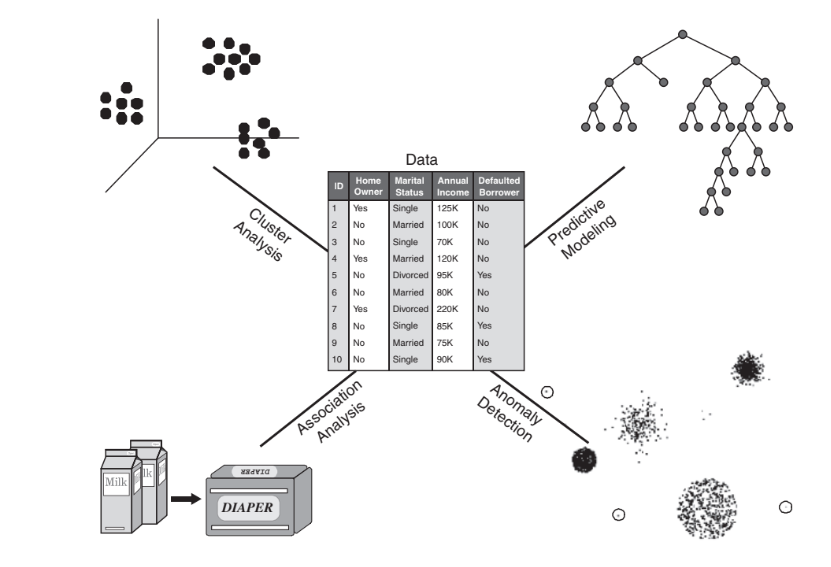
\includegraphics[width=10cm]{task.png}


\textbf{La modellazione predittiva} si riferisce al compito di costruire un modello per la variabile target
in funzione delle variabili esplicative. Ci sono due tipi di attività di modellazione predittiva: \underline{la classificazione}, utilizzata per classificare etichette discrete
 e \underline{la regressione}, che viene invece utilizzata per le variabili target continue. Per
esempio, prevedere se un utente Web effettuerà un acquisto online è un'attività di classificazione perché la variabile di destinazione è un valore binario.
D'altra parte, la previsione del prezzo futuro di un'azione è un compito di regressione
perché il prezzo è un valore continuo. L'obiettivo di entrambi i compiti è quello di
apprendere un modello che riduca al minimo l'errore tra i valori previsti e quelli reali
della variabile obiettivo.


\textbf{L'analisi delle associazioni} viene utilizzata per scoprire modelli che descrivono fortemente
caratteristiche associate ai dati. I modelli scoperti sono tipicamente rappresentati
sotto forma di regole di implicazione o sottoinsiemi di funzionalità. A causa dell'esponenziale
dimensione del suo spazio di ricerca, l'obiettivo dell'analisi di associazione è quello di estrarre il massimo
delle informazioni in modo efficiente. Utili applicazioni dell'analisi  delle associazioni
 includono la ricerca di gruppi di geni che hanno funzionalità correlate, identificare le pagine Web a cui si accede insieme o comprendere le relazioni
tra i diversi elementi del sistema climatico terrestre.



\textbf{L'analisi dei cluster} cerca di trovare gruppi di osservazioni strettamente correlate in modo che
le osservazioni che appartengono allo stesso cluster siano più simili tra loro
rispetto alle osservazioni che appartengono ad altri cluster. Clustering è stato utilizzato per
trovare gruppi di clienti correlati, trovare aree dell'oceano che hanno un significativo
impatto sul clima terrestre e comprimere i dati.



\textbf{Il rilevamento delle anomalie} è il compito di identificare le osservazioni le cui caratterestiche sono significativamente diverse dal resto dei dati. 
Tali osservazioni sono note come anomalie o valori anomali. L'obiettivo di un algoritmo di rilevamento delle anomalie
è scoprire le vere anomalie ed evitare di etichettare erroneamente oggetti normali come anomali. In altre parole, un buon rilevatore di anomalie deve avere un alto
tasso di rilevamento e un basso tasso di falsi allarmi. Applicazioni del rilevamento delle anomalie possono
includere il rilevamento di frodi, intrusioni di rete, modelli insoliti di malattie,
e disturbi dell'ecosistema, come siccità, inondazioni, incendi, uragani, ecc.
  \chapter{Preprocessing}
Vedere capitolo 2 del libro e riassumere le cose principali

  \chapter{Supervised learning}
  \chapter{Ensemble methods}
  \chapter{Neural Networks}
  \chapter{Clustering}
  
  % ... other parts
\end{document}
